\documentclass{article}
\usepackage[margin=0.5in]{geometry}
\usepackage{framed}
\usepackage{graphicx}
\usepackage{wrapfig}
\usepackage{listings}
\usepackage{amsmath, esint}
\usepackage{hyperref}
\usepackage{pdfpages}
\setlength{\parindent}{0cm}
\thispagestyle{empty}
\pagestyle{empty}
\newcommand{\Lagr}{\mathcal{L}}
\newcommand{\AnsLine}{\hspace{0.2 cm} \underline{\hspace{2 cm}}}
\newcommand{\Hgap}{\hspace{0.5cm}}
\newcommand{\Ihat}{\hat{i}}
\newcommand{\Jhat}{\hat{j}}
\newcommand{\Khat}{\hat{k}}
\newcommand{\Xhat}{\hat{x}}
\newcommand{\Yhat}{\hat{y}}
\newcommand{\Zhat}{\hat{z}}
\newcommand{\Nhat}{\hat{n}}
\newcommand{\DEL}{\vec{\nabla}}

\newcommand{\bfemph}[1]{\textbf{\emph{#1}}}

\setlength\parindent{0pt}
\def\changemargin#1#2{\list{}{\rightmargin#2\leftmargin#1}\item[]}
\let\endchangemargin=\endlist 

\title{\textbf{cMag:} A \emph{C} Version of the CLAS12 magnetic field package}

\author{D. Heddle  \\
	\emph{Christopher Newport University}  \\
         \emph{david.heddle@cnu.edu}\\
	}

\date{\today}

\begin{document}

\maketitle
\begin{abstract}
   The standard CLAS12 magnetic field that reads and interpolates the binary field maps for the solenoid and torus was written in JAVA. The package described here reproduces the same functionality in \emph{C}. That's  \emph{C}, not \emph{C++}, 
\footnote{The reason should be obvious. \emph{C} is the most beautiful programming language ever created while, remakably, \emph{C++} is the most hideous. This is not a matter of opinion.\\},\footnote{Pointer arithmetic, fine-grained control over memory (what could go wrong?), a preprocessor that allows you to hide critical code in inpenetrable macros, and a type-unsafe compiler that looks at your line of code that equates an integer pointer to an array of strings and says: \textit{``Cool, that works for me! I'm sure you know what you are doing."} I mean, how can you not love it!\\}
 but of course it can used in a \emph{C++} program. The most important feature is that it reads the same fieldmap files as the JAVA version. The code has been tested on OSX 10.15.4, ubuntu linux 20.04, and one other operating system. \footnote[666]{That would be Windows 10.}


\end{abstract}
\newpage

\tableofcontents
\newpage

\section {Introduction}
The magnetic field package used by \textit{ced} and by the CLAS12 reconstruction was written in JAVA. The  binary field map files used by the magnetic field package were written in JAVA\footnote{That's relevant, because JAVA specified that data be stored in big endian ordering on all platforms independent of architecture, while most of the machines we use in CLAS are little endian.\\}. However, the CLAS12 simulation, GEMC, is written in \textit{C++} and reads ascii field map files. In spite of great effort and testing, there is always a nagging suspicion that the simulation and reconstruction are using slightly different fields. This package, \textit{cMag}, was commisioned to solve that proble, so that GEMC could read the binary maps. However, \textit{cMag} goes beyond simply reading the maps, it also provides the same tri-linear interpolation access to the fields that the JAVA package uses. This may be of use to other \textit{C} and \textit{C++} CLAS12 developments. 

\section {Where do I get it?}
\subsection {The Code}
Like everything else that isn't available on \textit{Amazon}, the \textit{cMag} distribution is available on github at:
\newline
\newline
\url{https://github.com/heddle/cmag}.
\newline
\newline
\subsection {The Field Maps}
An exception to the rule stated above, the field maps are not available on either \textit{Amazon} or github. The field map files are not part of the \texttt{cMag} distribution \footnote{This is because some people are overly sensitive about having gigabytes of field map data stored in every CLAS12-related repository.\\}. They can be downloaded from here:\
\newline
\newline
 \url{https://clasweb.jlab.org/clas12offline/magfield/}.
\newline
\newline

\section {File Format}
Provided mostly for completeness, and demonstrating the raw power of \LaTeX, the fieldmap file format document has been inserted starting on the next page. If that doesn't work, the document is also included in the  \texttt{docs} directory of the \textit{cMag} distribution. \footnote{ As, self-rerentially, this document is, referring to the location where it is stored at the location where it is stored.}
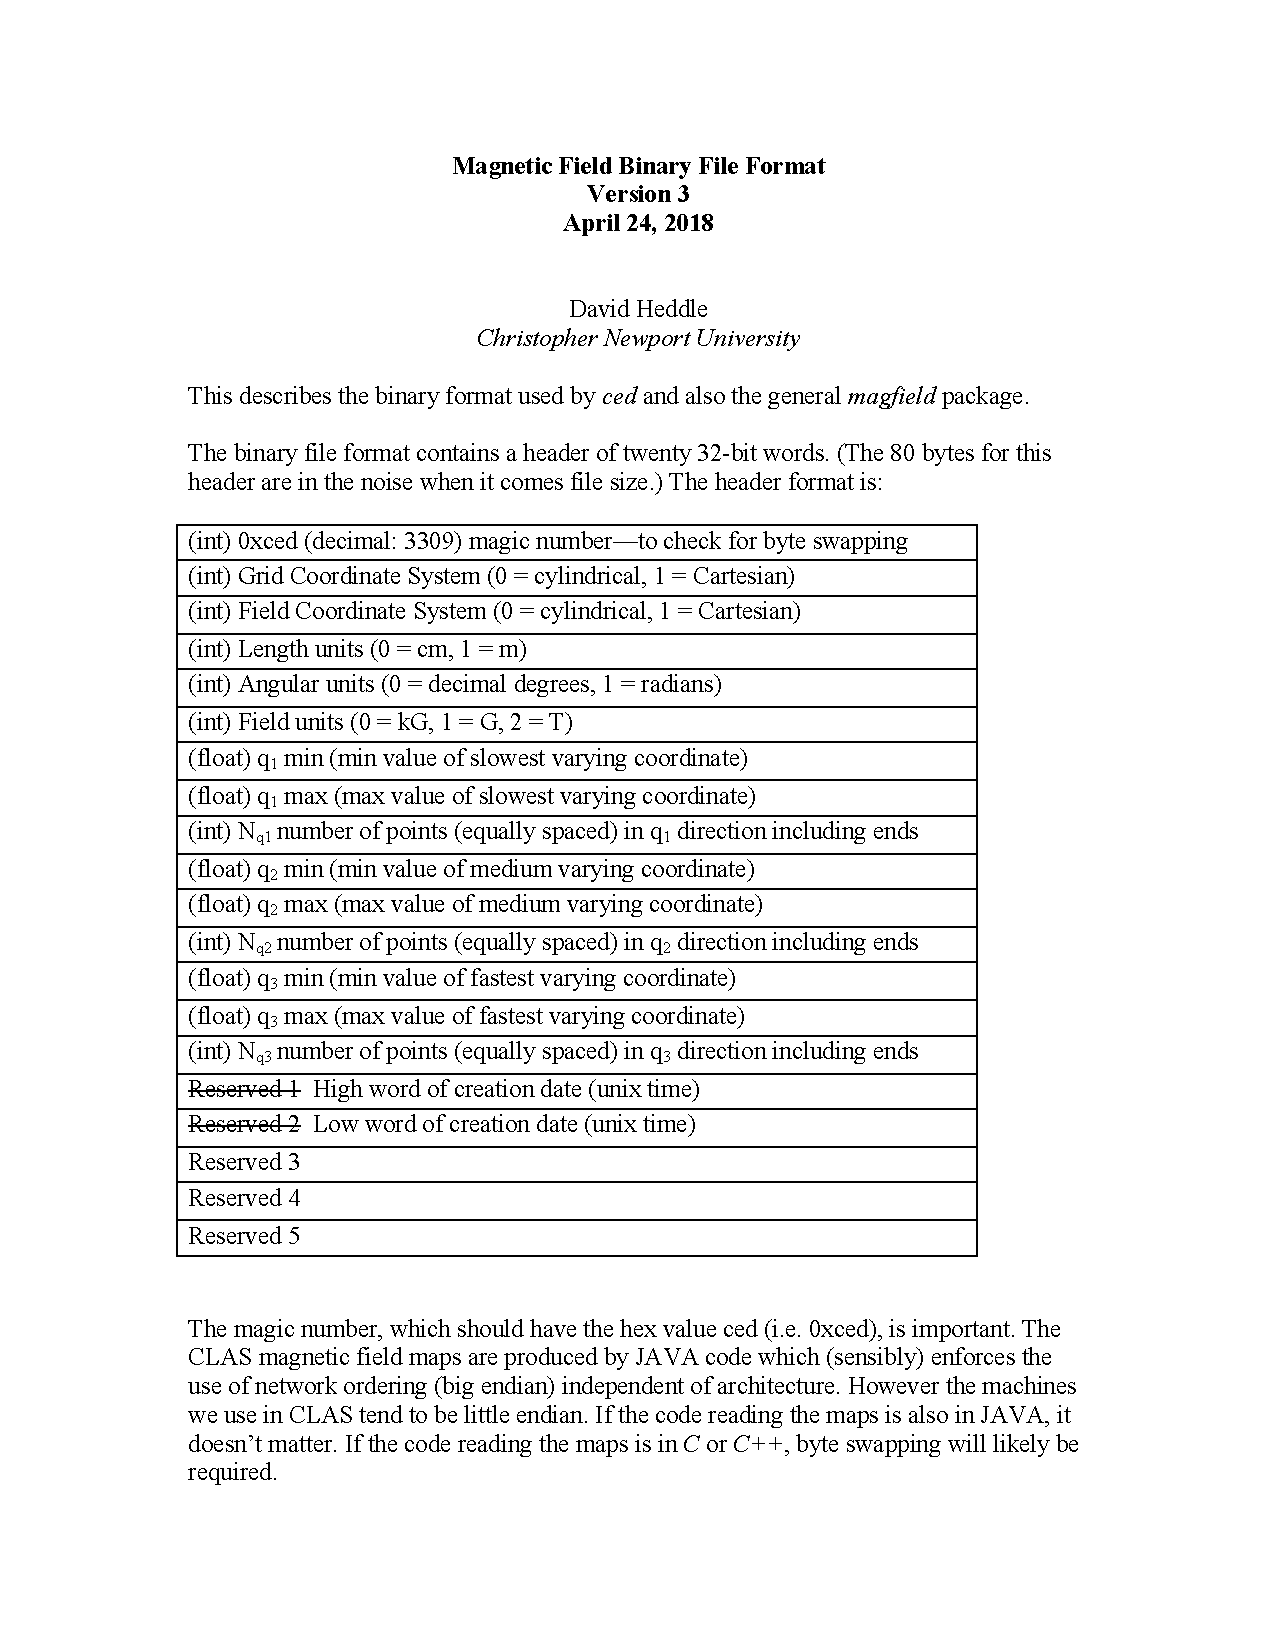
\includepdf[pages=-,pagecommand={},width=\textwidth]{FieldmapFileFormat.pdf}

\section {Building}
After cloning the \textit{cMag} repository, simply work your way down to the \texttt{src} folder where you will find a \texttt{Makefile}. Now, I have not written a makefile since CLAS was a 6 GeV toddler, but I do seem to recall that they are always very portable and never cause any grief. So I am comfortable that simply typing
\newline
\newline
\textbf{\texttt{\$make}}
\newline
\newline
will work on any platform. 
\newline
\newline
If it worked, you should now have toplevel \texttt{bin} and \texttt{lib} directories. Inside of \texttt{bin} should be an executable, \texttt{cMagTest}. Inside of \texttt{lib} should be the static library \texttt {libcMag.a}. Use that library, and the include files in the \texttt{includes} directory, to add the \text{cMag} functionality to your program.
\newline
\newline

\subsection {Unit Testing}
Assuming the build worked (and why shouldn't it?) the first thing you should do is run \texttt{bin/cMagTest} and see if it produces happy output (it does unit testing.) It will produce a \textit{lot} of output which you may or may not find interesting.  What you really care about is that \texttt{bin/cMagTest} terminates with the console print: 
\newline
\newline
\texttt{Program ran sucessfully. }
\newline
\newline
If one of the unit test fails it will say, well, something else, depending on which test failed first.
\section {Usage}
Assuming the build worked, and the testing was successful, you are ready to use the package. We will not discuss how to link it; you surely know how. We will discuss how to \textit{use} it after it has been successfuly  linked. Here we describe only the``public" functions, i.e. the ones you will likely use. Of course \textit{C}, being a highly democratic language, does not hide anything, so there are many more functions available, the functions that the``public" functions call upon. These functions  are accessible it you seek to cause mischief. 
\newline
\newline
We will begin with the first step, the initialization, which is the step that will most often go wrong. If you make it through the initialization, everything else should be smooth sailing.
\subsection{Initialization}


\end{document}
